\documentclass[12pt,letterpaper]{article}

\usepackage{amsfonts}
\usepackage{graphics}
\usepackage{graphicx}
\usepackage{colortbl}
\usepackage{amsmath}

\usepackage{algorithm}
\usepackage[noend]{algpseudocode}
\usepackage{array}

\usepackage{epstopdf}

\setlength\intextsep{10pt}
\setlength\textfloatsep{10pt}

\newenvironment{proof}{\noindent{\bf Proof:}}{\qed\bigskip}

\newtheorem{theorem}{Theorem}
\newtheorem{corollary}{Corollary}
\newtheorem{lemma}{Lemma} 
\newtheorem{claim}{Claim}
\newtheorem{fact}{Fact}
\newtheorem{definition}{Definition}
\newtheorem{assumption}{Assumption}
\newtheorem{observation}{Observation}
\newtheorem{example}{Example}
\newcommand{\qed}{\rule{7pt}{7pt}}

\newcommand{\assignment}[4]{
\thispagestyle{plain} 
\newpage
\setcounter{page}{1}
\noindent
\begin{center}
\framebox{ \vbox{ \hbox to 6.28in
{\bf CS578/STAT590: Introduction Machine Learning \hfill #1}
\vspace{4mm}
\hbox to 6.28in
{\hspace{2.5in}\large\mbox{Problem Set #2}}
\vspace{4mm}
\hbox to 6.28in
{{\it Handed Out: #3 \hfill Due: #4}}
}}
\end{center}
}

\newcommand{\solution}[4]{
\thispagestyle{plain} 
\newpage
\setcounter{page}{1}
\noindent
\begin{center}
\framebox{ \vbox{ \hbox to 6.28in
{\bf CS578/STAT590: Introduction to Machine Learning \hfill #4}
\vspace{4mm}
\hbox to 6.28in
{\hspace{2.5in}\large\mbox{Problem Set #3}}
\vspace{4mm}
\hbox to 6.28in
{#1 \hfill {\it Handed In: #2}}
}}
\end{center}
\markright{#1}
}



\def\Comment#1{\textsf{\textsl{$\langle\!\langle$#1\/$\rangle\!\rangle$}}}



\oddsidemargin 0in
\evensidemargin 0in
\textwidth 6.5in
\topmargin -0.5in
\textheight 9.0in

\begin{document}

\solution{Gen Nishida}{\today}{3}{Fall 2014}
% Fill in the above, for example, as follows:
% \solution{John Smith}{\today}{1}{Fall 2014}

\pagestyle{myheadings}  % Leave this command alone

\section{Questions}

\begin{enumerate}
\item Fitting an SVM classifier by hand (source: Machine Learning, a probabilistic perspective. K Murphy)

\begin{enumerate}
\item Write down a vector that is parallel to the optimal vector w.

The decision boundary is perpendicular to the vector $\phi(x_2)-\phi(x_1)$.
\[
\phi(x_2)-\phi(x_1)=[1, 2, 2]^T-[1, 0, 0]^T=[0, 2, 2]^T
\]
Thus, the vector that is parallel to the optimal vector $w$ is $[0, 1, 1]^T$.

\item What is the value of the margin that is achieved by this $w$?

The maximum margin is the half of the distance between two points in the 3d feature space. Thus,
\[
\frac{\|\phi(x_2)-\phi(x_1)\|}{2}=\frac{\|[0, 2, 2]^T\|}{2}=\sqrt{2}
\]

\item Solve for $w$, using the fact the margin is equal to $1/\|w\|$.

Let $w=k [0, 1, 1]^T$. Then,
\[
\|w\|=k\|[0, 1, 1]^T\|=\sqrt{2}k
\]
Since the maring is $\sqrt{2}$,
\[
\sqrt{2}=\frac{1}{\|w\|}=\frac{1}{\sqrt{2}k}
\]
By solving this, we obtain $k=1/2$. Thus, $w=[0, 1/2, 1/2]^T$.

\item Solve for $w_0$ using your value for $w$ and Equations 1 to 3.

By substituting $w$ of Equations 2 and 3, we get
\[
\begin{cases}
y_1(w^T\phi(x_1)+w_0)=-([0, 1/2, 1/2]^T \cdot [1, 0, 0]^T+w_0)=-w_0\ge 1 \\
y_2(w^T\phi(x_2)+w_0)=([0,1/2,1/2]^T \cdot [1, 2, 2]^T+w_0)=2+w_0\ge 1
\end{cases}
\]
By solving this, we obtain
\[
-1\le w_0 \le -1
\]
Thus, $w_0=-1$.

\item Write down the form of the discriminant function $f(x)=w_0+w^T\phi(x)$ as an explicit function of $x$.

\[
f(x)=w_0 + w^T \phi(x)=-1 + [0, 1/2, 1/2]^T \cdot [1, \sqrt{2}x, x^2]^T=\frac{1}{2}x^2+\frac{1}{\sqrt{2}}x-1
\]

\end{enumerate}

\item We define a concept space C that consists of the union of $k$ disjoint intervals in a real line. A concept in C is represented therefore using $2k$ parameters: $a_1 \le b_1 \le a_2 \le b_2 \le \cdots \le a_k \le b_k$. An example (a real number) is classified as positive by such concept iff it lies in one of the intervals. Give the VC dimension of H (and prove its correctness).

The answer is $2k$.

{\bf Proof:}

Let $VC(k)$ be the VC dimension for $k$ disjoint intervals in a real line. I prove by indiction that $VC(k)=2k$ in the following. When $k=1$, two examples have four patterns in total, and all the cases can be correctly classified (Figure.\ref{fig:vc_dimension1}). Thus, $VC(1)=2$, which satisifies my hypothesis. 

\begin{figure}[hbtp]
\centering
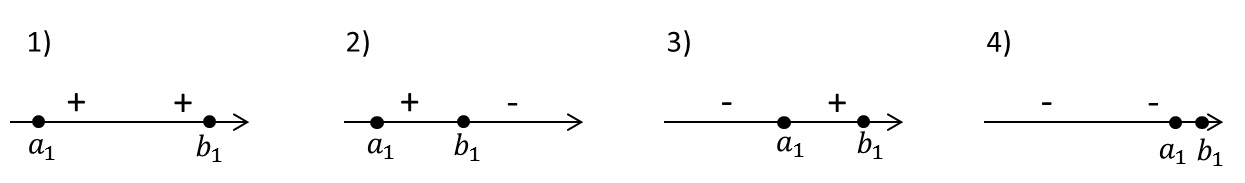
\includegraphics[width=150mm]{vc_dimension1.jpg}
\caption{For the case of $k=1$, two examples are correctly classified in all the four cases. Thus, $VC(1)=2$.}
\label{fig:vc_dimension1}
\end{figure}

Given that $VC(k-1)=2(k-1)$, we want to show that two additional examples can be correctly separated by an additional interval. Here, we do not lose generalization even if we assume that two additional examples are greater than the existing $2(k-1)$ examples that are already correctly classified. Then, there are only four cases in terms of the labels of two additional examples, and the two additional examples are correctly classified by the additional interval in all the cases (Figure. \ref{fig:vc_dimension2}). Thus, 
\[
VC(k)=VC(k-1)+2=2(k-1)+2=2k
\]
Therefore, $VC(k)=2k$ by induction.

\begin{figure}[hbtp]
\centering
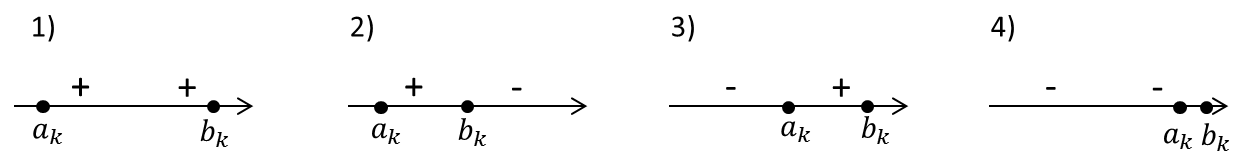
\includegraphics[width=150mm]{vc_dimension2.jpg}
\caption{When adding $k$-th interval, two additional examples are correctly classified in all the four cases. Thus, $VC(k)=VC(k-1)+2$.}
\label{fig:vc_dimension2}
\end{figure}

\item The Gradient Descent (GD) algorithm

\begin{enumerate}
\item Write in one sentence: what are the hyper parameters of the GD algorithm.

The hyper parameters are the initial weight vector which you can randomly initialize if you want, learning rate that is the step size of updating the weight vector, a parameter $\lambda$ that defines the impact of the regularizer, and the convergence criteria when to stop the iteration such as the maximum number of iterations.

\item Write in one sentence: What is the difference between $l1$ and $l2$ regularization.

$l1$ regularization uses $l1$ norm as the regularization term, which encourages the sparsity, while $l2$ regularization uses $l2$ norm.

\item Write down the gradient descent algorithm applied to hinge loss with $l2$ regularization.

\begin{algorithm}
\caption{Gradient descent algorithm applied to hige loss with l2 regularization}\label{euclid}
\begin{algorithmic}[1]
\Procedure{GradientDescent()}{}
\State Initialize $w^{(0)}$ randomly
\For{$i=0$ to $T$}
\State $\Delta w=(0, \cdots, 0)$
\ForAll{training data $x_d$ for $d = 1,\cdots,D$}
\ForAll{component $w_j$ for $j = 1, \cdots,N$}
\If{$y_d w^{(i)} \cdot x_d > 1$}
\State $\Delta w_j+=0$
\Else
\State $\Delta w_j+=\eta y_d x_{dj}$
\EndIf
\EndFor
\EndFor
\ForAll{component $w_j$ for $j = 1, \cdots,N$}
\State $\Delta w_j-=\eta \lambda w_j$
\EndFor
\State $w^{(i+1)}=w^{(i)}+\Delta w$
\State \Return $w^{(i+1)}$ when it has converted
\EndFor
\EndProcedure
\end{algorithmic}
\end{algorithm}


\end{enumerate}



\end{enumerate}

\section{Programming Assignment}

\end{document}

